322. Серёжа согнул две проволоки так, как показано на рисунке, и наложил их друг на друга, не разгибая. Какова наибольшая возможная длина их общей (совпавшей) части, если 2 клеточки равны 1 см?\\
\begin{figure}[ht!]
\center{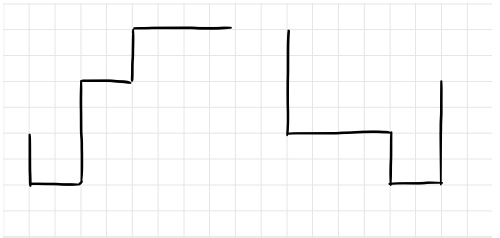
\includegraphics[scale=0.35]{prov1.png}}
\end{figure}\\
